% InitialPage for tecnic documents
%
% This command allows to create an initial page with a defined layout. In order
% to create the page following data must be given:
% - Author: given with \author command;
% - Title: given with \title command;
\makeatletter
\newcommand{\initialpagetecnicdocument}{
\pagenumbering{gobble}
\newgeometry{left=7.5cm} %defines the geometry for the titlepage
\pagecolor{niceblue}
\noindent
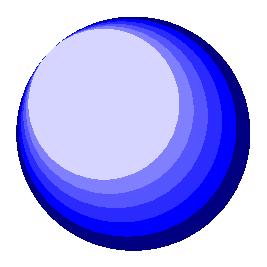
\includegraphics[width=4cm]{logo.eps}\\[-1em]
{\color{white}
\makebox[0pt][l]{\rule{1.3\textwidth}{1pt}}
\par
\noindent
\textbf{\textsf{WTeam Tecnical Document}} \\ {\color{titlecolor}\textsf{Author: \@author}}
\vfill
\noindent
{\huge \textsf{\@title}}
\vskip\baselineskip
\noindent
\textsf{\@date}
\restoregeometry
\nopagecolor}
\pagenumbering{arabic}}
\makeatother

%%% Emphasis %%%
\newcommand{\emphasis}[1]{\emph{#1}}

%% Inline code %%%
% This is a command for writing a line of code directly inside a paragraph. I's
% useful for writing a command or a function name.
\newcommand{\inlinecode}[1]{\texttt{#1}}


